% ------------------------------------------------------------------------------
% TYPO3 Version 9.1 - What's New - Chapter "Introduction" (English Version)
%
% @author	Michael Schams <schams.net>
% @license	Creative Commons BY-NC-SA 3.0
% @link		http://typo3.org/download/release-notes/whats-new/
% @language	English
% ------------------------------------------------------------------------------
% LTXE-CHAPTER-UID:		7fdf26cc-362160ab-d6c8b905-19722b20
% LTXE-CHAPTER-NAME:	Introduction
% ------------------------------------------------------------------------------

\section{Introduction}
\begin{frame}[fragile]
	\frametitle{Introduction}

	\begin{center}\huge{Introduction}\end{center}
	\begin{center}\huge{\color{typo3darkgrey}\textbf{The Facts}}\end{center}

\end{frame}

% ------------------------------------------------------------------------------
% LTXE-SLIDE-START
% LTXE-SLIDE-UID:		db9ce9bf-51fe8c3b-c6a2649f-aa7018b5
% LTXE-SLIDE-TITLE:		TYPO3 Version 9.1 - The Facts
% ------------------------------------------------------------------------------
\begin{frame}[fragile]
	\frametitle{Introduction}
	\framesubtitle{TYPO3 Version 9.1 - The Facts}

	\begin{itemize}
		\item Release date: 30 January 2018
		\item Release type: Sprint Release
	\end{itemize}

	\begin{figure}
		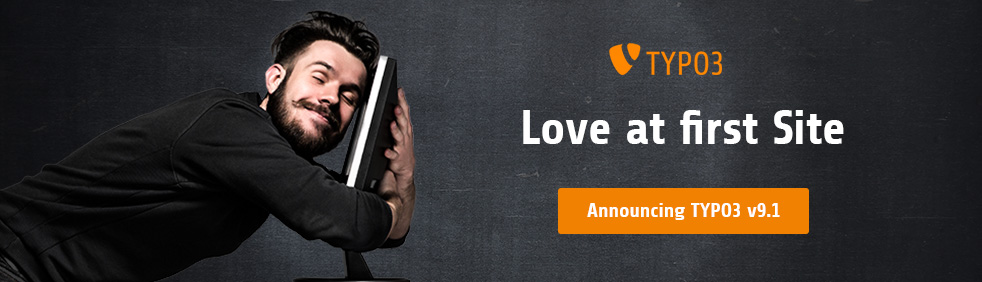
\includegraphics[width=0.95\linewidth]{Introduction/typo3-v91-banner.jpg}
	\end{figure}

\end{frame}

% ------------------------------------------------------------------------------
% LTXE-SLIDE-START
% LTXE-SLIDE-UID:		baf0e8fa-b8335fbe-911020ab-489d6156
% LTXE-SLIDE-TITLE:		System Requirements
% ------------------------------------------------------------------------------
\begin{frame}[fragile]
	\frametitle{Introduction}
	\framesubtitle{System Requirements}

	\begin{itemize}
		\item PHP version 7.2\newline
			\smaller
				(will possibly be lowered to PHP 7.1 or 7.0 for future releases, decision pending)
			\normalsize

		\item PHP settings:

			\begin{itemize}
				\item \texttt{memory\_limit} >= 128M
				\item \texttt{max\_execution\_time} >= 240s
				\item \texttt{max\_input\_vars} >= 1500
				\item compilation option \texttt{-}\texttt{-disable-ipv6} must \underline{not} be used
			\end{itemize}

		\item Most database servers supported by \textbf{Doctrine DBAL} also work with TYPO3.
			Tested DB engines are for example:
	\end{itemize}

	\begin{figure}
		
\includegraphics[width=0.70\linewidth]{Introduction/logo-databases.png}
	\end{figure}

\end{frame}

% ------------------------------------------------------------------------------
% LTXE-SLIDE-START
% LTXE-SLIDE-UID:		dfe5c3a8-72a55162-da879770-778ebfec
% LTXE-SLIDE-TITLE:		Development, Release and Maintenance Timeline
% ------------------------------------------------------------------------------
\begin{frame}[fragile]
	\frametitle{Introduction}
	\framesubtitle{Development, Release and Maintenance Timeline}

	\textbf{TYPO3 v9}

	\begin{figure}
		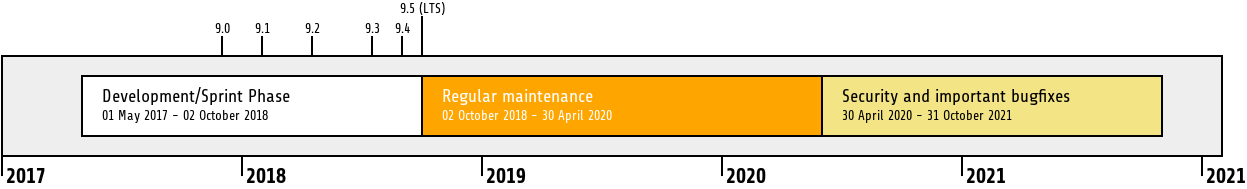
\includegraphics[width=1\linewidth]{Introduction/typo3-v9-lifecycle.png}
	\end{figure}

	\textbf{Extended Support}\newline
	\smaller
		The \href{https://typo3.com}{TYPO3 GmbH} offers further support options
		for TYPO3 v9 LTS even after 31 October 2021 for up to two additional
		years.
	\normalsize

%	\url{https://typo3.com/our-services/extended-support/}

\end{frame}

% ------------------------------------------------------------------------------
% LTXE-SLIDE-START
% LTXE-SLIDE-UID:		1c2b096f-e4e0a65c-b0b0d84b-e18889a1
% LTXE-SLIDE-TITLE:		TYPO3 v9 Roadmap
% ------------------------------------------------------------------------------
\begin{frame}[fragile]
	\frametitle{Introduction}
	\framesubtitle{TYPO3 v9 Roadmap}

	Estimated release dates and their primary focus:

	\begin{itemize}

		\item v9.0 \tabto{1.1cm}12/Dec/2017\tabto{3.4cm}Install Tool and Page Tree Refactoring,\newline
			\tabto{3.4cm}Unified Page Translations
		\item
			\begingroup
				\color{typo3orange}
					v9.1 \tabto{1.1cm}30/Jan/2018\tabto{3.4cm}Redirect Handling
			\endgroup
		\item v9.2 \tabto{1.1cm}10/Apr/2018\tabto{3.4cm}Site Configuration
		\item v9.3 \tabto{1.1cm}12/Jun/2018\tabto{3.4cm}URL Routing
		\item v9.4 \tabto{1.1cm}04/Sep/2018\tabto{3.4cm}Frontend Editing
		\item v9.5 \tabto{1.1cm}02/Oct/2018\tabto{3.4cm}LTS Release

	\end{itemize}

	\smaller
		\url{https://typo3.org/news/article/typo3-v9-roadmap/}
	\normalsize

\end{frame}

% ------------------------------------------------------------------------------
% LTXE-SLIDE-START
% LTXE-SLIDE-UID:		27b13d1c-5c952e3e-d4422d93-0a8a273d
% LTXE-SLIDE-TITLE:		Installation
% ------------------------------------------------------------------------------
\begin{frame}[fragile]
	\frametitle{Introduction}
	\framesubtitle{Installation}

	\begin{itemize}
		\item Official \textit{classic} installation procedure under Linux/Mac OS X\newline
			(DocumentRoot for example \texttt{/var/www/site/htdocs}):
		\begin{lstlisting}
			$ cd /var/www/site
			$ wget --content-disposition get.typo3.org/9.1
			$ tar xzf typo3_src-9.1.0.tar.gz
			$ cd htdocs
			$ ln -s ../typo3_src-9.1.0 typo3_src
			$ ln -s typo3_src/index.php
			$ ln -s typo3_src/typo3
			$ touch FIRST_INSTALL
		\end{lstlisting}

		\item Symbolic links under Microsoft Windows:

			\begin{itemize}
				\item Use \texttt{junction} under Windows XP/2000
				\item Use \texttt{mklink} under Windows Vista and Windows 7 and higher
			\end{itemize}

	\end{itemize}
\end{frame}

% ------------------------------------------------------------------------------
% LTXE-SLIDE-START
% LTXE-SLIDE-UID:		2991c08b-8831f59c-56bc188c-e05b8e92
% LTXE-SLIDE-TITLE:		Installation using composer
% ------------------------------------------------------------------------------
\begin{frame}[fragile]
	\frametitle{Installation and Upgrade}
	\framesubtitle{Installation Using \texttt{composer}}

	\begin{itemize}
		\item Installation using \textit{composer} under Linux/Mac OS X

			\begin{lstlisting}
				$ cd /var/www/site/
				$ composer create-project typo3/minimal
			\end{lstlisting}

		\item Alternatively, create your custom \texttt{composer.json} file and run:

			\begin{lstlisting}
				$ composer install
			\end{lstlisting}

			An example \texttt{composer.json} file can be downloaded at:\newline
			\small
				\href{https://git.typo3.org/TYPO3CMS/Distributions/Base.git/blob/HEAD:/composer.json}{git.typo3.org/TYPO3CMS/Distributions/Base.git/blob/HEAD:/composer.json}
			\normalsize

	\end{itemize}
\end{frame}

% ------------------------------------------------------------------------------
% LTXE-SLIDE-START
% LTXE-SLIDE-UID:		3bc1e21e-cf2c23c4-b1d641af-8e351b92
% LTXE-SLIDE-TITLE:		Upgrade to TYPO3 Version 9
% ------------------------------------------------------------------------------
%\begin{frame}[fragile]
%	\frametitle{Introduction}
%	\framesubtitle{Upgrade to TYPO3 Version 9.x}
%
%	\begin{itemize}
%		\item Upgrades only possible from TYPO3 v8 LTS
%		\item TYPO3 < v8 LTS should be updated to TYPO3 v8 LTS first
%	\end{itemize}
%
%	\begin{itemize}
%
%		\item Upgrade instructions:\newline
%			\smaller\url{https://wiki.typo3.org/Upgrade#Upgrading_to_9.1}\normalsize
%		\item Official TYPO3 guide "TYPO3 Installation and Upgrading":
%			\smaller\url{https://docs.typo3.org/typo3cms/InstallationGuide}\normalsize
%		\item General approach:
%			\begin{itemize}
%				\item Check minimum system requirements \small(PHP, MySQL, etc.)
%				\item Review \textbf{deprecation\_*.log} in old TYPO3 instance
%				\item Update all extensions to the latest version
%				\item Deploy new sources and run Install Tool -> Upgrade Wizard
%				\item Review startup module for backend users (optionally)
%			\end{itemize}
%	\end{itemize}
%
%\end{frame}
%
% ------------------------------------------------------------------------------
